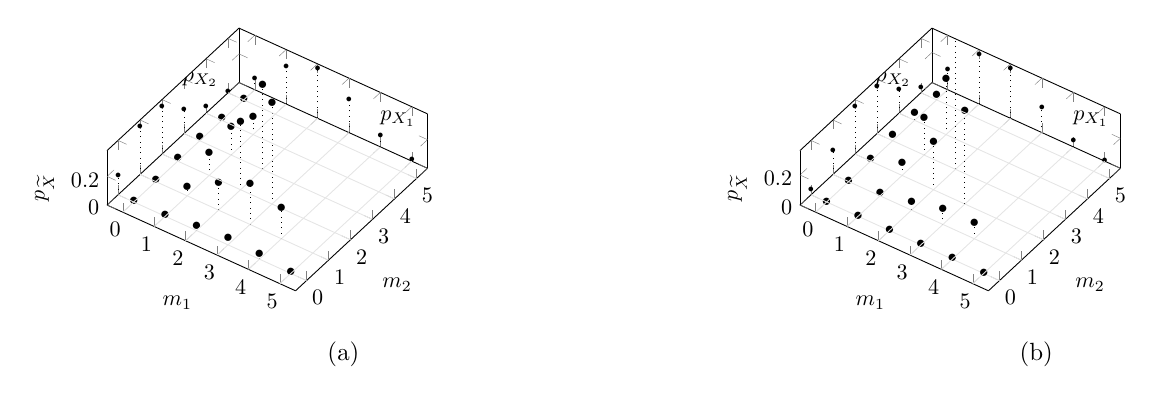
\begin{tikzpicture}[scale=.8]
\shorthandoff{>}
%
%
\pgfmathsetmacro{\n}{5};% numeros para la multinomial
\pgfmathsetmacro{\dec}{.5};% shitf para dibujar las marginales
%
% Ejemplo [6 5 4]/15
\begin{scope}
%
\pgfmathsetmacro{\pu}{2/5};% p_1
\pgfmathsetmacro{\pd}{1/3};% p_2
\pgfmathsetmacro{\qu}{floor((\n+1)*\pu)};% modo de la binomial 1
\pgfmathsetmacro{\qd}{floor((\n+1)*\pd)};% modo de la binomial 2
\pgfmathsetmacro{\mau}{factorial(\n)/factorial(\qu)/factorial(\n-\qu)*(\pu^\qu)*((1-\pu)^(\n-\qu))};% maximo de la binomial 1
\pgfmathsetmacro{\mad}{factorial(\n)/factorial(\qd)/factorial(\n-\qd)*(\pd^\qd)*((1-\pd)^(\n-\qd))};% maximo de la binomial 2
\pgfmathsetmacro{\ma}{max(\mau,\mad)};% maximo de ambas binomiales
%
\begin{axis}[
    colormap = {whiteblack}{color(0cm)  = (white);color(1cm) = (black)},
    width=.55\textwidth,
    view={35}{70},
    enlargelimits=false,
    xmin={-\dec},
    xmax={\n+\dec},
    ymin={-\dec},
    ymax={\n+\dec},
    zmax={1.1*\ma},
    color=black,
    xtick={0,...,\n},
    ytick={0,...,\n},
    xlabel=$m_1$,
    ylabel=$m_2$,
    zlabel=$p_{\widetilde{X}}$,
]
%
\pgfmathsetmacro{\bu}{(1-\pu-\pd)^\n};% coeficiente binomial por la probabilidad p1
\pgfmathsetmacro{\bd}{\bu};% coeficiente binomial por la probabilidad p2
%
\pgfmathsetmacro{\bmu}{(1-\pu)^\n};% lo mismo para la marginale 1
\pgfmathsetmacro{\bmd}{(1-\pd)^\n};% lo mismo para la marginale 2
%
\foreach \mu in {0,...,\n} {
  \foreach \md in {0,...,\n} {
    \ifnum \numexpr\mu+\md < \numexpr\n+1
      \addplot3 [dotted,domain=0:\bd,samples=2, samples y=0,color=black] (\mu,\md,\x)  node[scale=.85]{$\bullet$};
      %
      \pgfmathsetmacro{\bld}{\bd*\pd*(\n-\md)/((\md+1)*(1-\pu-\pd))};
      \global\let\bd\bld;% proba en m2 (m1 fijo) actualizado
    \fi
  }
  %
  % Marginales
  \addplot3 [dotted,domain=0:\bmu,samples=2, samples y=0,color=black] (\mu,{\n+\dec},\x)  node[scale=.55]{$\bullet$};
  \addplot3 [dotted,domain=0:\bmd,samples=2, samples y=0,color=black] ({-\dec},\mu,\x)  node[scale=.55]{$\bullet$};
  %
  % lineas (m1,m2) abajo
  \addplot3 [domain={-\dec}:{\n+\dec},samples=2, samples y=0,color=black!10] (\mu,\x,0);
  \addplot3 [domain={-\dec}:{\n+\dec},samples=2, samples y=0,color=black!10] (\x,\mu,0);
  %
  \pgfmathsetmacro{\blu}{\bu*\pu*(\n-\mu)/((\mu+1)*(1-\pu-\pd))};
  \global\let\bu\blu;\global\let\bd\blu;% proba inicial en m1 actualizada
  %
  % lo mismo para cada marginal
  \pgfmathsetmacro{\blmu}{\bmu*\pu*(\n-\mu)/((\mu+1)*(1-\pu))};
  \global\let\bmu\blmu;% proba 1 actualizada
  \pgfmathsetmacro{\blmd}{\bmd*\pd*(\n-\mu)/((\mu+1)*(1-\pd))};
  \global\let\bmd\blmd;% proba 2 actualizada
}
%
\node at (axis cs:{3*\n/4},{\n+\dec},{\mau/2})[right]{$p_{X_1}$};
\node at (axis cs:{-\dec},{3*\n/4},{\mad/2})[above]{$p_{X_2}$};
\end{axis}
\node at ({3*\n/4},-1)[scale=.9]{(a)};
\end{scope}
%
%
%
%
% Ejemplo [1 1 1]/3
\begin{scope}[xshift = 11cm]
%
\pgfmathsetmacro{\pu}{1/3};% p_1
\pgfmathsetmacro{\pd}{1/2};% p_2
\pgfmathsetmacro{\qu}{floor((\n+1)*\pu)};% modo de la binomial 1
\pgfmathsetmacro{\qd}{floor((\n+1)*\pd)};% modo de la binomial 2
\pgfmathsetmacro{\mau}{factorial(\n)/factorial(\qu)/factorial(\n-\qu)*(\pu^\qu)*((1-\pu)^(\n-\qu))};% maximo de la binomial 1
\pgfmathsetmacro{\mad}{factorial(\n)/factorial(\qd)/factorial(\n-\qd)*(\pd^\qd)*((1-\pd)^(\n-\qd))};% maximo de la binomial 2
\pgfmathsetmacro{\ma}{max(\mau,\mad)};% maximo de ambas binomiales
%
\begin{axis}[
    colormap = {whiteblack}{color(0cm)  = (white);color(1cm) = (black)},
    width=.55\textwidth,
    view={35}{70},
    enlargelimits=false,
    xmin={-\dec},
    xmax={\n+\dec},
    ymin={-\dec},
    ymax={\n+\dec},
    zmax={1.1*\ma},
    color=black,
    xtick={0,...,\n},
    ytick={0,...,\n},
    xlabel=$m_1$,
    ylabel=$m_2$,
    zlabel=$p_{\widetilde{X}}$,
]
%
\pgfmathsetmacro{\bu}{(1-\pu-\pd)^\n};% coeficiente binomial por la probabilidad p1
\pgfmathsetmacro{\bd}{\bu};% coeficiente binomial por la probabilidad p2
%
\pgfmathsetmacro{\bmu}{(1-\pu)^\n};% lo mismo para la marginale 1
\pgfmathsetmacro{\bmd}{(1-\pd)^\n};% lo mismo para la marginale 2
%
\foreach \mu in {0,...,\n} {
  \foreach \md in {0,...,\n} {
    \ifnum \numexpr\mu+\md < \numexpr\n+1
      \addplot3 [dotted,domain=0:\bd,samples=2, samples y=0,color=black] (\mu,\md,\x)  node[scale=.85]{$\bullet$};
      %
      \pgfmathsetmacro{\bld}{\bd*\pd*(\n-\md)/((\md+1)*(1-\pu-\pd))};
      \global\let\bd\bld;% proba en m2 (m1 fijo) actualizado
    \fi
  }
  %
  % Marginales
  \addplot3 [dotted,domain=0:\bmu,samples=2, samples y=0,color=black] (\mu,{\n+\dec},\x)  node[scale=.55]{$\bullet$};
  \addplot3 [dotted,domain=0:\bmd,samples=2, samples y=0,color=black] ({-\dec},\mu,\x)  node[scale=.55]{$\bullet$};
  %
  % lineas (m1,m2) abajo
  \addplot3 [domain={-\dec}:{\n+\dec},samples=2, samples y=0,color=black!10] (\mu,\x,0);
  \addplot3 [domain={-\dec}:{\n+\dec},samples=2, samples y=0,color=black!10] (\x,\mu,0);
  %
  \pgfmathsetmacro{\blu}{\bu*\pu*(\n-\mu)/((\mu+1)*(1-\pu-\pd))};
  \global\let\bu\blu;\global\let\bd\blu;% proba inicial en m1 actualizada
  %
  % lo mismo para cada marginal
  \pgfmathsetmacro{\blmu}{\bmu*\pu*(\n-\mu)/((\mu+1)*(1-\pu))};
  \global\let\bmu\blmu;% proba 1 actualizada
  \pgfmathsetmacro{\blmd}{\bmd*\pd*(\n-\mu)/((\mu+1)*(1-\pd))};
  \global\let\bmd\blmd;% proba 2 actualizada
}
%
\node at (axis cs:{3*\n/4},{\n+\dec},{\mau/2})[right]{$p_{X_1}$};
\node at (axis cs:{-\dec},{3*\n/4},{\mad/2})[above]{$p_{X_2}$};
\end{axis}
\node at ({3*\n/4},-1)[scale=.9]{(b)};
\end{scope}
%
\end{tikzpicture}